\section{Microarchitectural Attack Surface Analysis}
\frame{\sectionpage}

\begin{frame}{Attack Surface Richness in the CPU Pipeline}
    \begin{itemize}
        \item CPUs break down instructions into micro-operations. 
        \item These micro-operations take place in dozens or even hundreds of CPU subsystems!
    \end{itemize}
    \begin{figure}
        \centering
        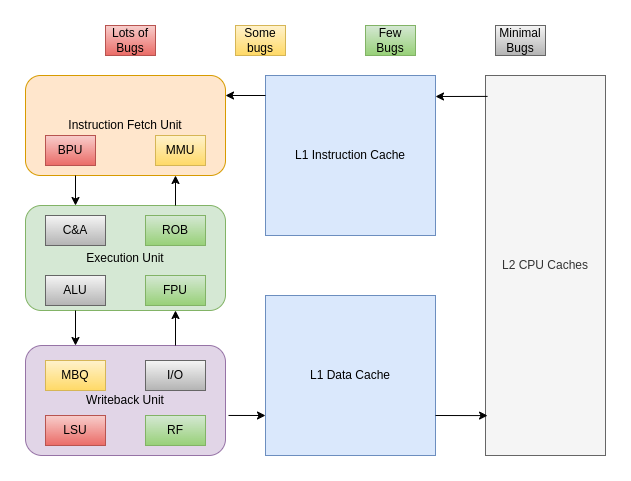
\includegraphics[width=0.7\textwidth, height=5cm]{images/cpu_diagram_border.png}
        \caption{Simple Fetch-Execute-Write pipeline and historical tendencies for CPU bugs.}
        \label{fig:few-cpu-diagram}
    \end{figure}
    \note{
        \begin{itemize}
            \item TODO: Replace this awful ugly graphic.
            \item Acronyms,
            \begin{itemize}
                \item BPU = Branch Predictor Unit
                \item MMU = Memory Management Unit (Translation Lookaside Buffers (TLBs), Page Table Walkers (PTWs), etc. )
                \item C\&A = Coprocessors and Accelerators
                \item ROB = Re-order Buffer
                \item ALU = Arithmetic Logic Unit
                \item FPU = Floating Point Unit
                \item MBQ = ??? = Memory Buses and Queues?? 
                \item I/O = Input/Output
                \item LSU = Load/Store Unit
                \item RF  = Register File
            \end{itemize}
        \end{itemize}
    }
\end{frame}

\begin{frame}{Branch Predictor Unit}{Exploited in \hyperlink{spectre}
{{\color{pink}\textit{Spectre}}} and \href{https://ileakage.com/}{\color{pink}\textit{iLeakage}}}
    \begin{columns}
        \begin{column}{0.7\textwidth}
            \begin{itemize}
                \item   A branch predictor is a subsystem which attempts to identify the direction the instruction pointer will go on CPU branches.
                \item \textit{Static} branch prediction uses a fixed set of rules to guess which codepath comes next.
                \item \textit{Dynamic} branch prediction uses previous branches to determine which codepath comes next.
            \end{itemize}
        \end{column}
        \begin{column}{0.3\textwidth}
            \begin{figure}
                \centering
                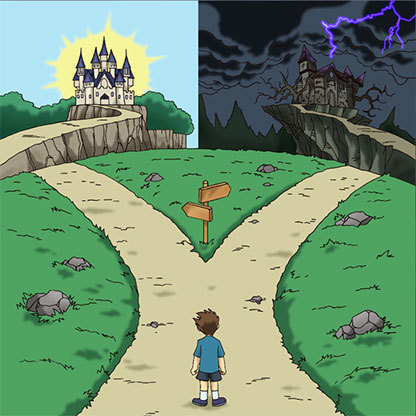
\includegraphics[width=\textwidth]{images/two-paths.jpg}
                \label{fig:branch-predictor-meme}
            \end{figure}
        \end{column}
    \end{columns}
    Attackers can reliably control the branch predictor, so processors must be very careful what they do during speculation!
    \note{
        \begin{itemize}
            \item Speculation refers to the instructions that the processor "guesses" during branch prediction. These are also referred to as \textit{transient instructions} or wholly \textit{transient execution}.
            \item The branch predictor is and out-of-order execution aren't really in a dedicated box in a particular core. Their "placement" is very design specific. 
        \end{itemize}
    }
\end{frame}

\begin{frame}{Load-store Unit}{Exploited in \href{https://publications.cispa.saarland/3924/1/security_risc.pdf}{\color{pink}\textit{A Security RISC}}}
    \begin{block}{What is a Load-store Unit?}
        The Load-store unit is a processor subsystem responsible for interacting with memory and the register file (RF). It typically interconnects with the L1-Caches, which then connect to the rest of the cache hierarchy. LSUs organize and tag cache metadata using hash functions. Cache timing side channels are historically the richest attack surface for microarchitectural bugs.
    \end{block}
    Classical attacks on LSUs include, 
    \begin{itemize}
        \item \href{https://eprint.iacr.org/2005/271.pdf}{\color{pink}Prime+Probe}, the "original" attack on AES S-boxes via priming a shared cache with an eviction set, then probing to see which parts of the GF(256) Table were indexed.
        \item \href{https://www.usenix.org/system/files/conference/usenixsecurity14/sec14-paper-yarom.pdf}{\color{pink}Flush+Reload}, where an attacker flushes the last-level cache using the \textit{clflush} instruction, then times the differences of memory accesses of a victim process. 
    \end{itemize}
    \note{
        \begin{itemize}
            \item Load-store units are historically the single richest attack surface for microarchitectural bugs.
            \item LSUs also suffer a lot from bus interconnects, cache hierarchies, and are often more on the "SoC" level than the "CPU" level.
            \item Attacks like Rowhammer are really more about the memory, and so are not really covered in this talk or via the LSU.
            \item You'll see Prime+Probe and Flush+Reload in particular discussed in modern works as primitives. They're kind of like heap grooming techniques on a microarchitectural level.
        \end{itemize}
    }
\end{frame}

\begin{frame}{ReOrder Buffer and Out-of-order Machine}{Exploited in \href{https://meltdownattack.com/meltdown.pdf}{\color{pink}\textit{Meltdown}} and \href{https://foreshadowattack.eu/foreshadow.pdf}{\color{pink}\textit{Foreshadow}}}
    \begin{itemize}
        \item The ReOrder Buffer (RoB) reconciles operations from out-of-order execution. It is oftentimes more problematic in CISC architectures, such as the \href{https://bughunters.google.com/blog/5997221712101376/the-reptar-cpu-vulnerability}{\color{pink}Reptar} vulnerability.
    \end{itemize}
    \begin{figure}
        \centering
        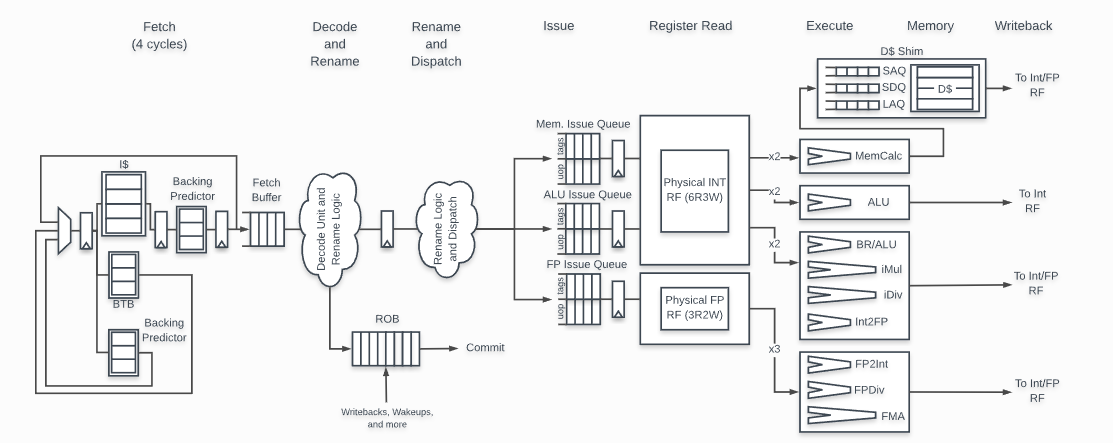
\includegraphics[width=0.77\textwidth]{images/boom_pipeline_simplified.png}
        \caption{Simplified pipeline of the \href{https://docs.boom-core.org/en/latest/sections/intro-overview/boom-pipeline.html}{\color{pink}Chipyard BOOM} architecture.}
        \label{fig:chipyard-boom-pipeline}
    \end{figure}
    \note{
        \begin{itemize}
            \item Reptar is pretty crazy, it's theoretically possible to take it all the way to code execution.
            \item At a high-level, Reptar is a bug in some Intel chips where "rep" prefixed instructions aren't queued properly, so the instruction pointer kinda goes all over the place, and the out-of-order machine is never really reordered.
        \end{itemize}
    }
\end{frame}

\begin{frame}{Everything else!}
    There's no shortage of vulnerable subsystems inside of CPUs!
    \begin{block}{Floating Point Units}
        Often in RISC architectures, floating point operations may not be constant time, introducing side-channels. In the infamous \href{https://en.wikipedia.org/wiki/Pentium_FDIV_bug}{\color{pink}Intel Penitum FDIV bug}, divisions could be outright wrong!
    \end{block}
    \begin{block}{Line Fill Buffers}
        An intermediate memory and caching subsystem in Intel Skylake architecture exploited in the \href{https://www.ieee-security.org/TC/SP2019/papers/588.pdf}{\color{pink}Rogue In-flight Data Load} attacks.
    \end{block}
    \begin{block}{Register File}
        Certain registers, exposed in the ISA or otherwise, may be able to access data at times or places they're not supposed to. This is the case in the AMD \href{https://github.com/google/security-research/blob/master/pocs/cpus/zenbleed/}{\color{pink}Zenbleed} attack. 
    \end{block}
    \note{
        \begin{itemize}
            \item Many of these intermediate buffers and structures have come under attack since RIDL; attacks that focus on these subsystems are largely called "Microarchitectural Data Sampling" or "MDS" attacks.
            \item Historically, these attacks are actually among the most exploitable. They tend to have reliable non-probabilistic properties, which is quite nice for exploitation. 
            \item The processor doesn't allow even the kernel to read from these internal hardware subsystems, so attackers usually have to side-channel data from them, often with the help of transient execution.
        \end{itemize}
    }
\end{frame}